\chapter{Risultati, conclusioni e lavori futuri}
\section{Simulazioni}
In questa sezione vengono presentati i risultati delle simulazioni effettuate e i loro valori.
\subsection{Simulazione 1}\label{sim1}
I valori di questa simulazione\space \cref{fig:sim1} sono:
\begin{itemize}
    \item Numero di nodi: 500
    \item \texttt{sniffThreshold}: 1.5
    \item \texttt{wiggleBias}: 0
    \item \texttt{evaporation}: 0.6
    \item \texttt{diffusion}: 0.5
    \item \texttt{deposit}: 1
    \item \texttt{startX}: -15
    \item \texttt{startY}: -15
    \item \texttt{width}: 30
    \item \texttt{height}: 30
    \item \texttt{step}: 0.5
    \item \texttt{customDiffusionTreshold}: 5
\end{itemize}
\begin{figure}[ht]
    \centering
    \subfigure[]{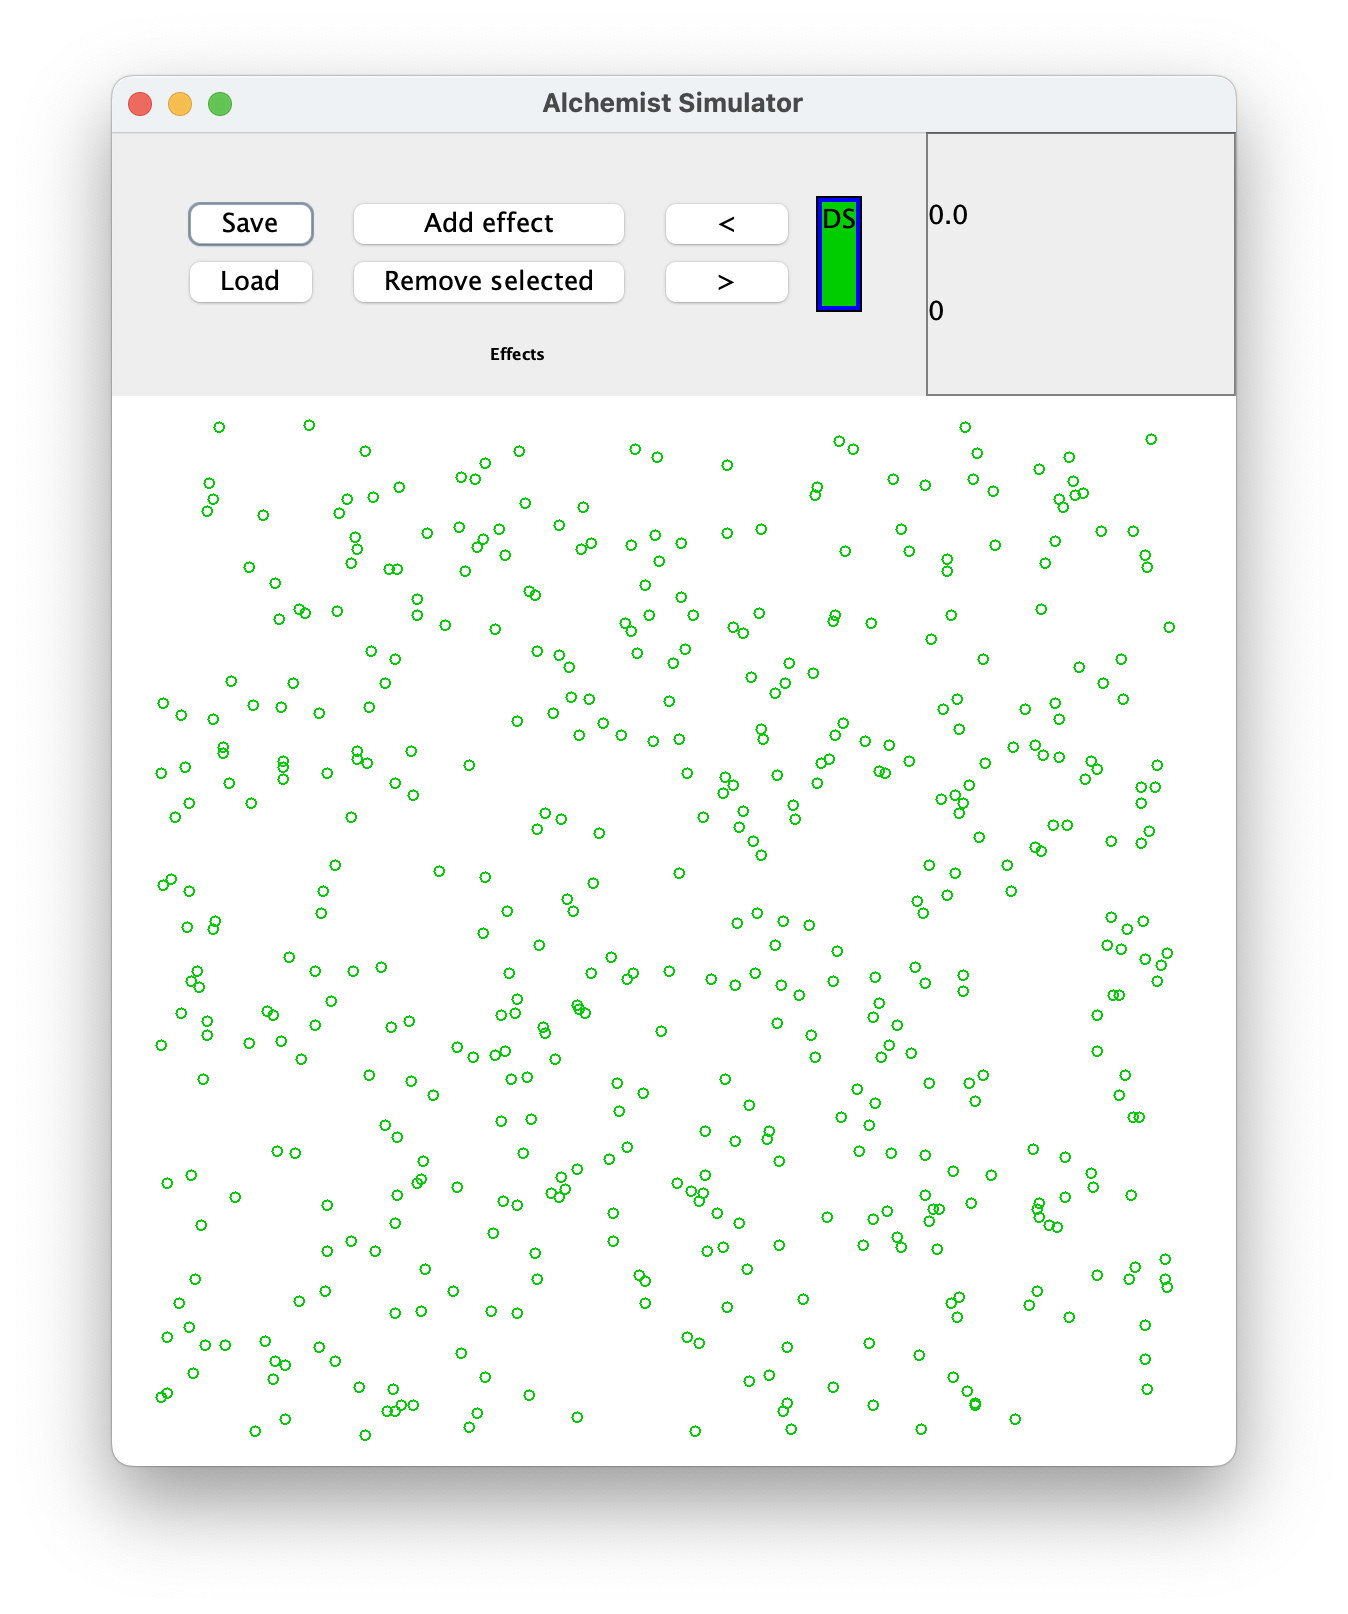
\includegraphics[width=0.32\textwidth]{figures/rect0.png}} 
    \subfigure[]{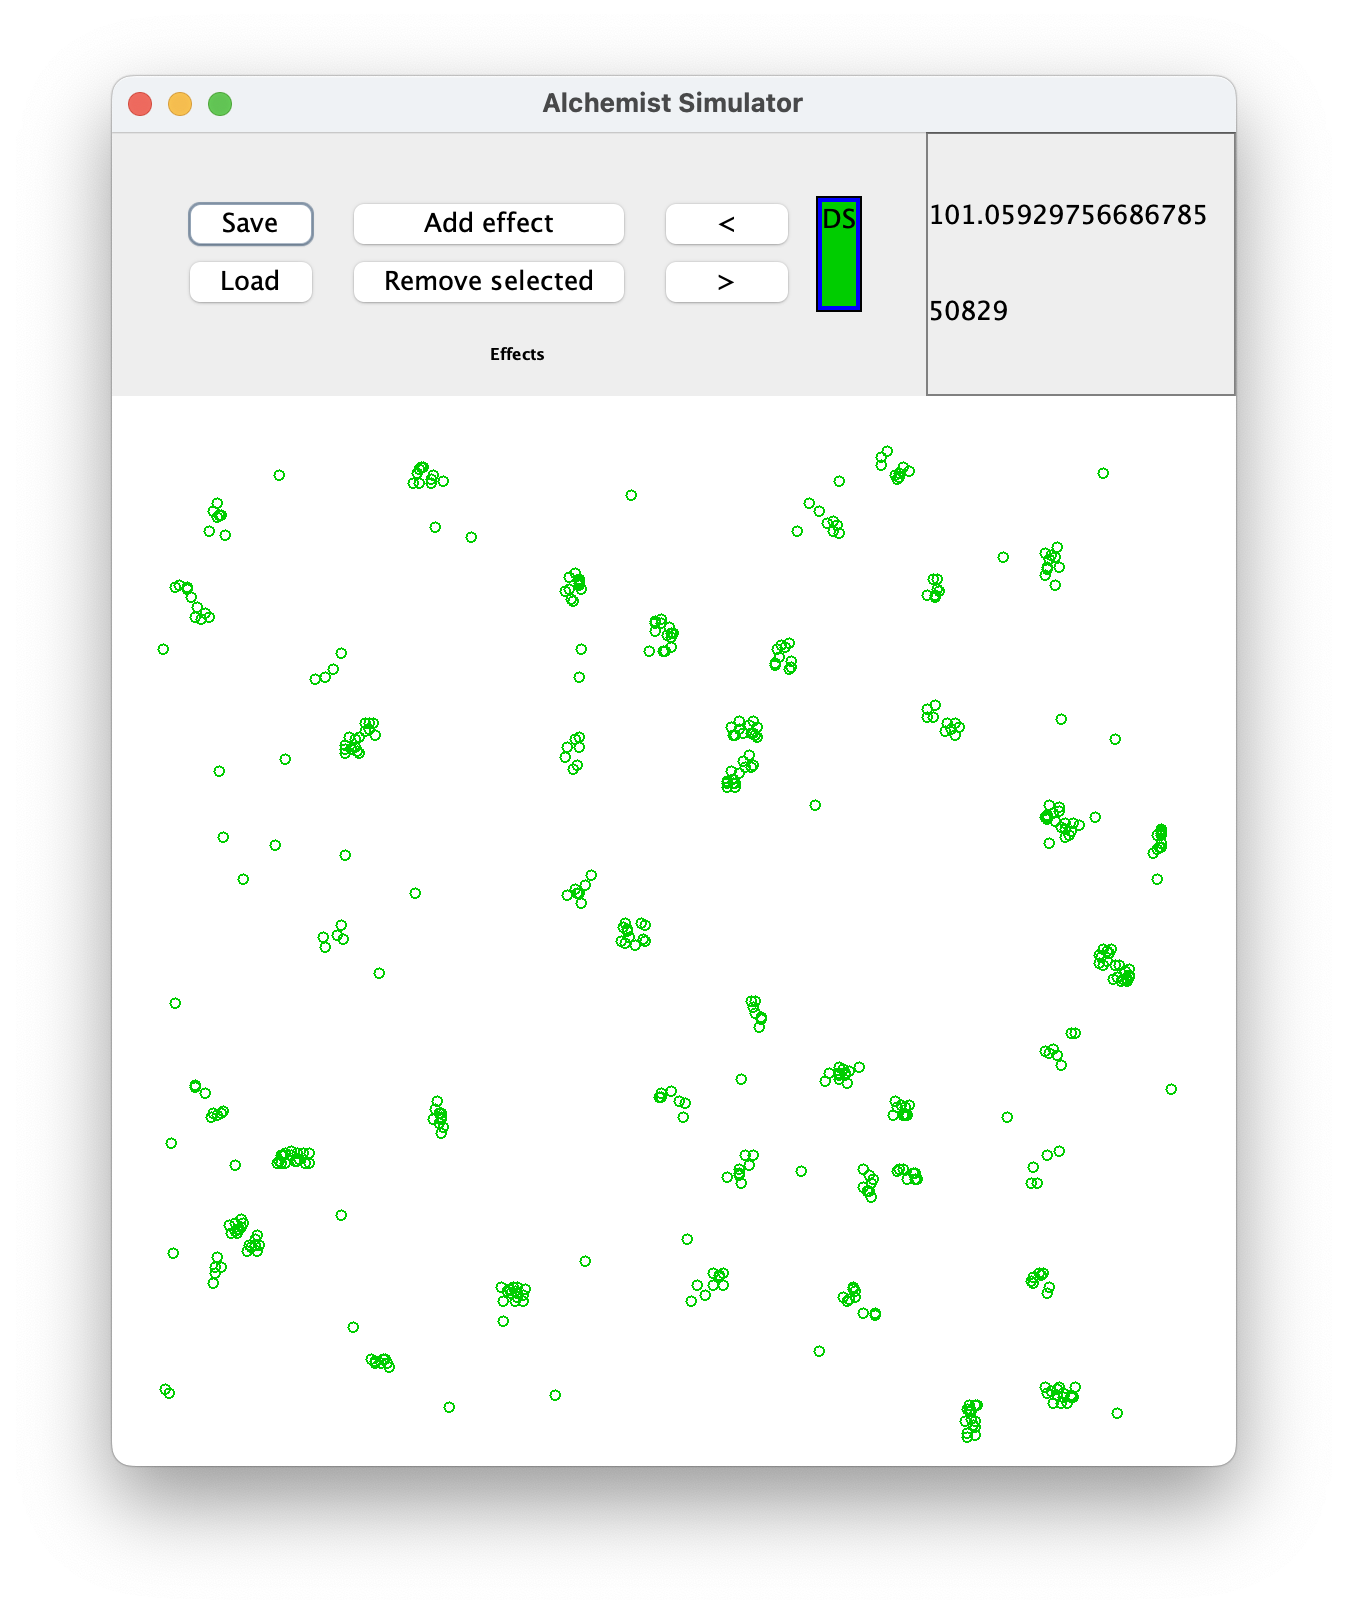
\includegraphics[width=0.32\textwidth]{figures/rect100.png}} 
    \subfigure[]{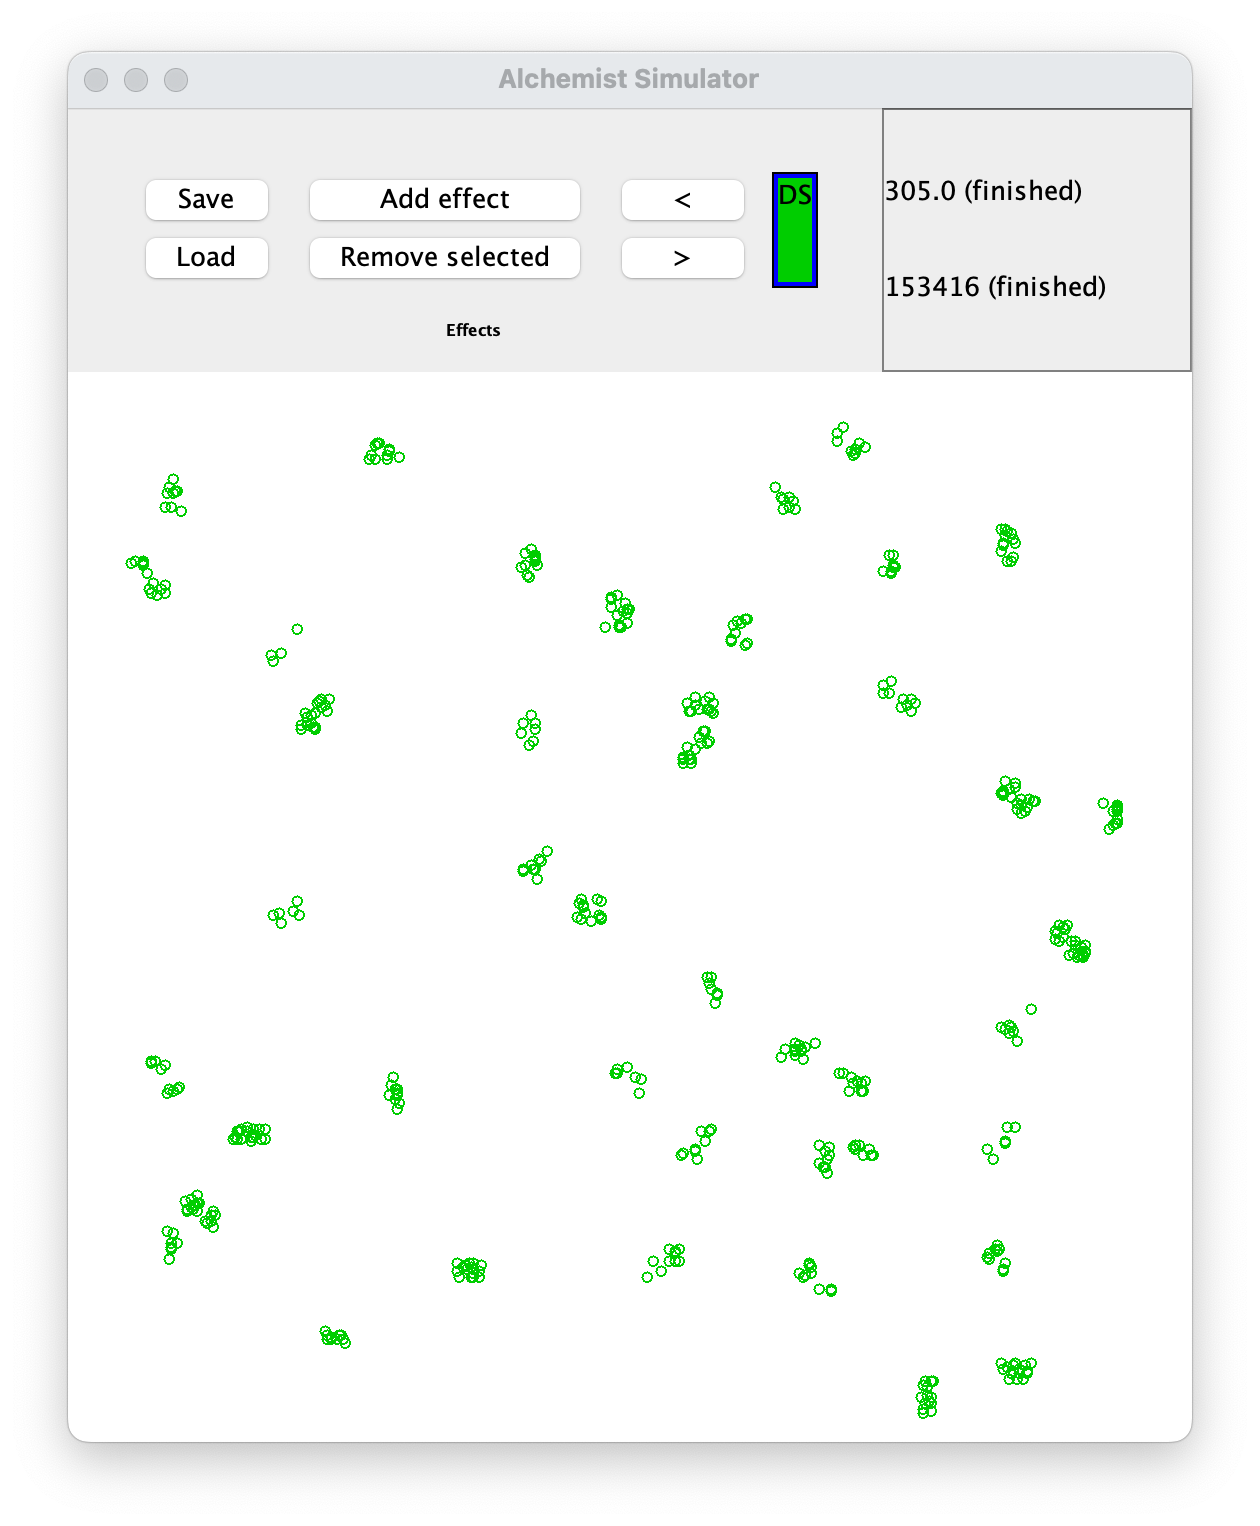
\includegraphics[width=0.32\textwidth]{figures/rectFine.png}}
    \caption{(a) Inizio (b) Dopo 100 secondi (c) Dopo 300 secondi}\label{fig:sim1}
\end{figure}

\subsection{Simulazione 2}\label{sim2}
I valori di questa simulazione\space \cref{fig:sim2} sono:
\begin{itemize}
    \item Numero di nodi: 500
    \item \texttt{sniffThreshold}: 4
    \item \texttt{wiggleBias}: 0
    \item \texttt{evaporation}: 0.6
    \item \texttt{diffusion}: $\frac{1}{18}$
    \item \texttt{deposit}: 1
    \item \texttt{startX}: -15
    \item \texttt{startY}: -15
    \item \texttt{width}: 30
    \item \texttt{height}: 30
    \item \texttt{step}: 0.5
    \item \texttt{customDiffusionTreshold}: 1
\end{itemize}
\begin{figure}[ht]
    \centering
    \subfigure[]{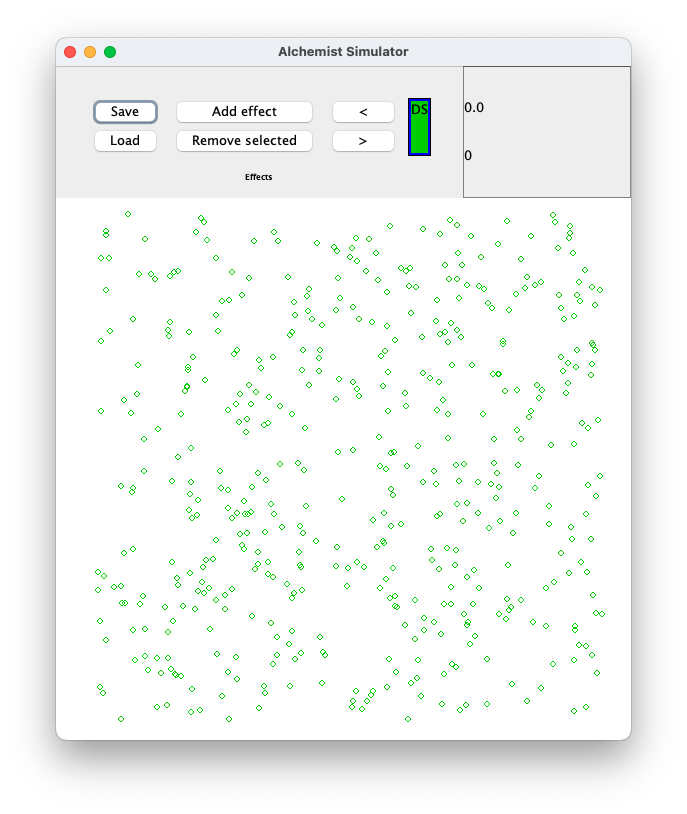
\includegraphics[width=0.32\textwidth]{figures/slow0.png}} 
    \subfigure[]{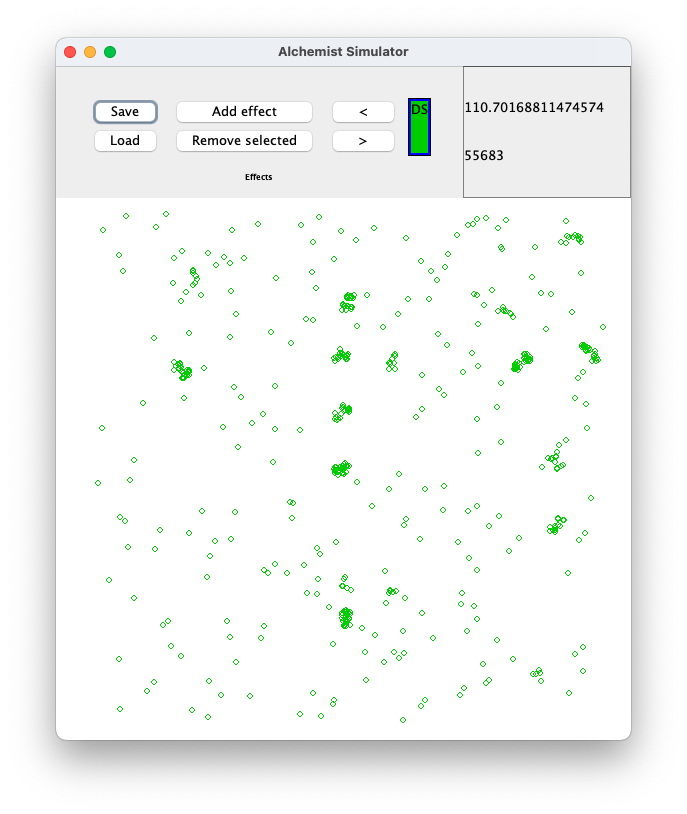
\includegraphics[width=0.32\textwidth]{figures/slow100.png}} 
    \subfigure[]{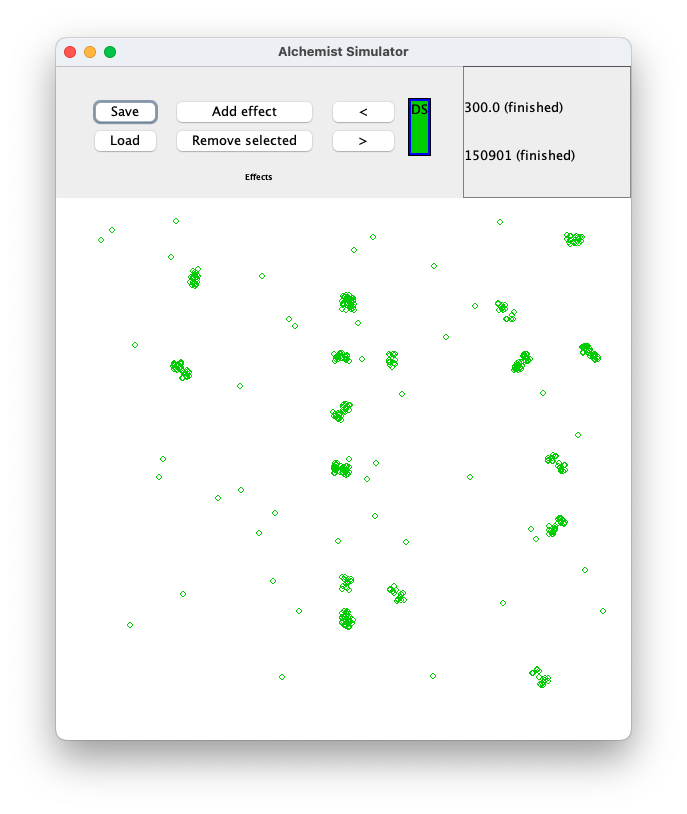
\includegraphics[width=0.32\textwidth]{figures/slowF.png}}
    \caption{(a) Inizio (b) Dopo 100 secondi (c) Dopo 300 secondi}\label{fig:sim2}
\end{figure}

\subsection{Simulazione 3}\label{sim3}
I valori di questa simulazione\space \cref{fig:sim3} sono:
\begin{itemize}
    \item Numero di nodi: 100
    \item \texttt{sniffThreshold}: 1.5
    \item \texttt{wiggleBias}: 0
    \item \texttt{evaporation}: 0.6
    \item \texttt{diffusion}: 0.5
    \item \texttt{deposit}: 1
    \item \texttt{startX}: -15
    \item \texttt{startY}: -15
    \item \texttt{width}: 30
    \item \texttt{height}: 30
    \item \texttt{step}: 0.5
    \item \texttt{customDiffusionTreshold}: 5
\end{itemize}
\begin{figure}[ht]
    \centering
    \subfigure[]{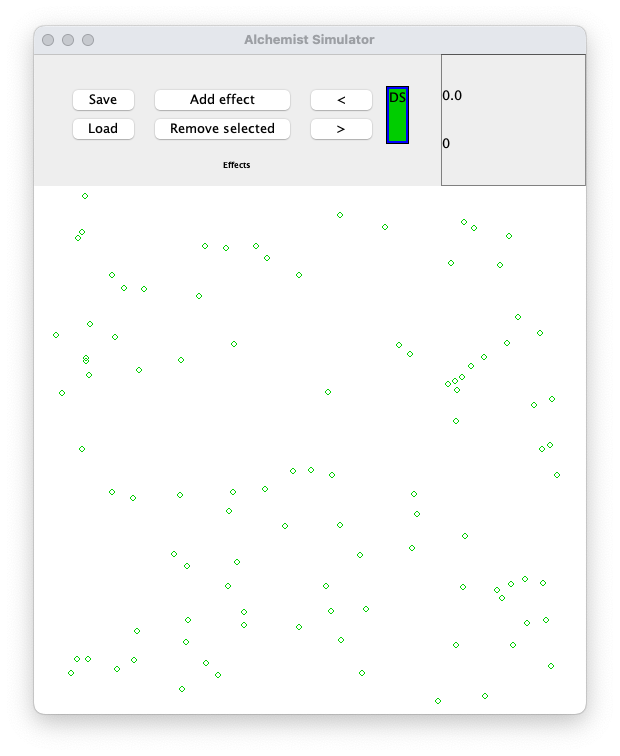
\includegraphics[width=0.32\textwidth]{figures/cento0.png}} 
    \subfigure[]{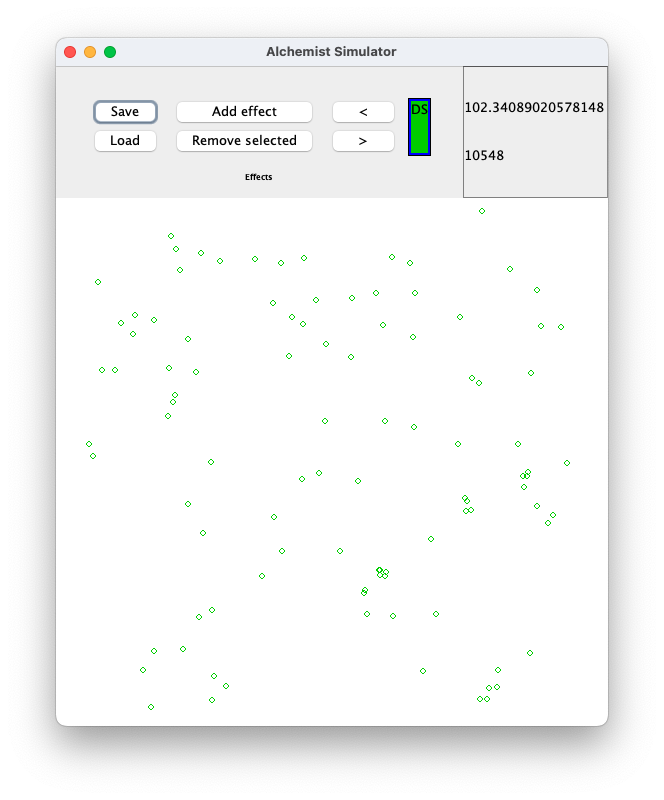
\includegraphics[width=0.32\textwidth]{figures/cento100.png}} 
    \subfigure[]{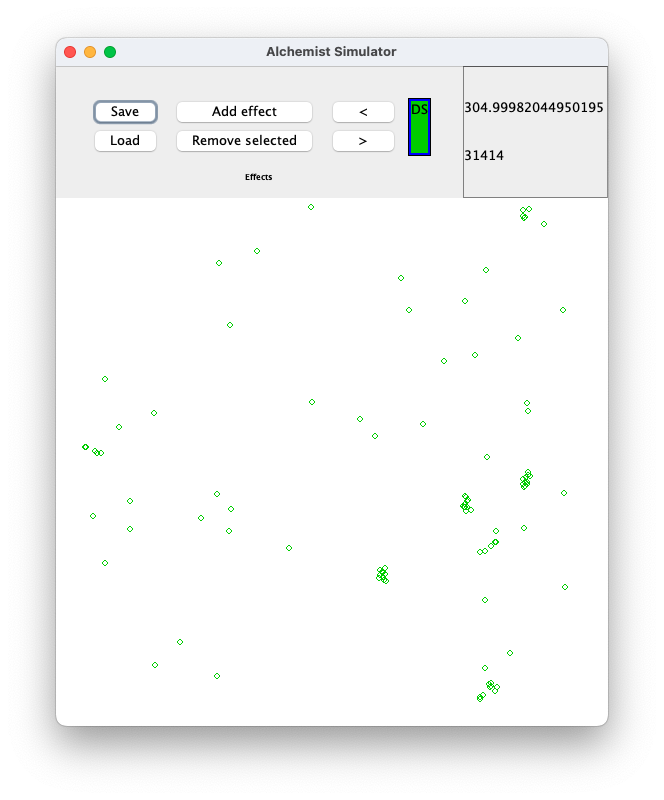
\includegraphics[width=0.32\textwidth]{figures/centoF.png}}
    \caption{(a) Inizio (b) Dopo 100 secondi (c) Dopo 300 secondi}\label{fig:sim3}
\end{figure}

\subsection{Simulazione 4}\label{sim4}
I valori di questa simulazione\space \cref{fig:sim4} sono:
\begin{itemize}
    \item Numero di nodi: 100
    \item \texttt{sniffThreshold}: 4
    \item \texttt{wiggleBias}: 0
    \item \texttt{evaporation}: 0.6
    \item \texttt{diffusion}: $\frac{1}{18}$
    \item \texttt{deposit}: 1
    \item \texttt{startX}: -15
    \item \texttt{startY}: -15
    \item \texttt{width}: 30
    \item \texttt{height}: 30
    \item \texttt{step}: 0.5
    \item \texttt{customDiffusionTreshold}: 1
\end{itemize}
\begin{figure}[ht]
    \centering
    \subfigure[]{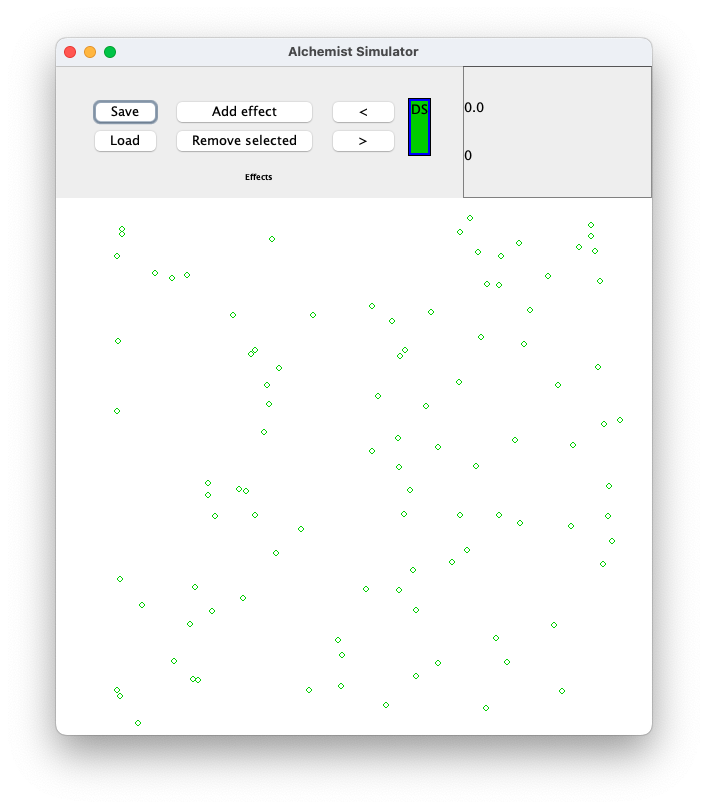
\includegraphics[width=0.32\textwidth]{figures/centoNo0.png}} 
    \subfigure[]{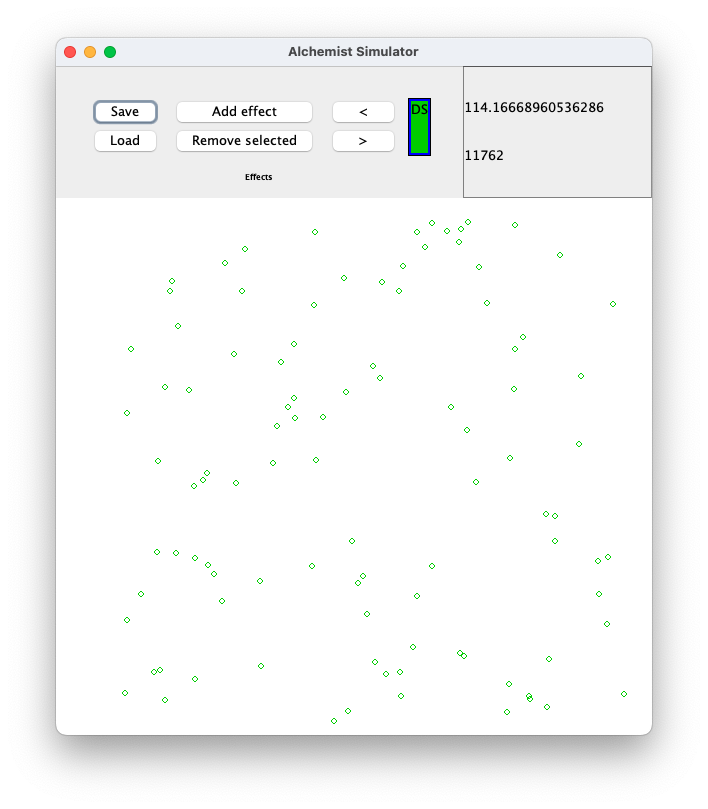
\includegraphics[width=0.32\textwidth]{figures/centoNo100.png}} 
    \subfigure[]{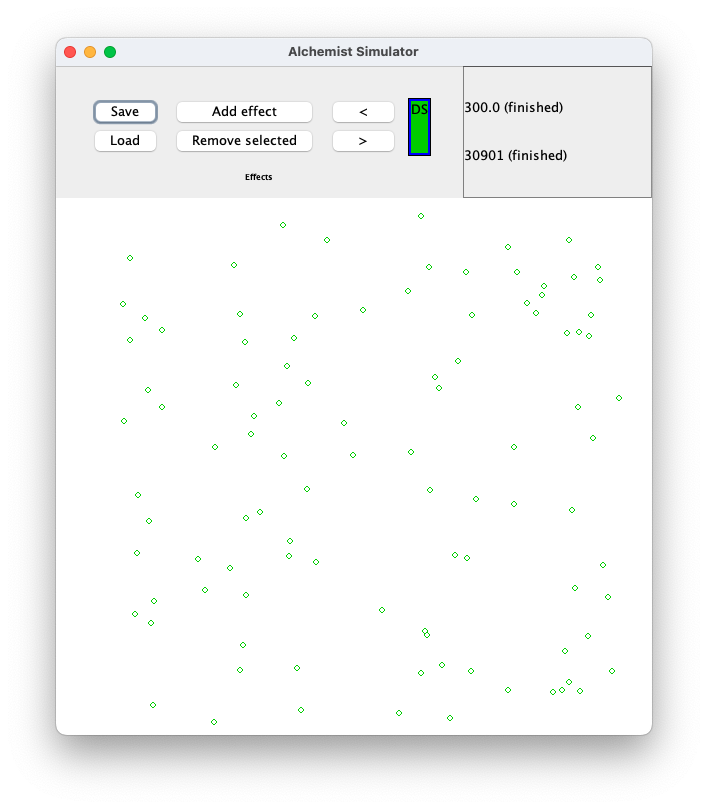
\includegraphics[width=0.32\textwidth]{figures/centoNoF.png}}
    \caption{(a) Inizio (b) Dopo 100 secondi (c) Dopo 300 secondi}\label{fig:sim4}
\end{figure}

\subsection{Simulazione 5}\label{sim5}
I valori di questa simulazione\space \cref{fig:sim5} sono:
\begin{itemize}
    \item Numero di nodi: 500
    \item \texttt{sniffThreshold}: 4
    \item \texttt{wiggleBias}: 0
    \item \texttt{evaporation}: 0.5
    \item \texttt{diffusion}: 1
    \item \texttt{deposit}: 2
    \item \texttt{startX}: -10
    \item \texttt{startY}: -10
    \item \texttt{width}: 20
    \item \texttt{height}: 20
    \item \texttt{step}: 0.5
    \item \texttt{customDiffusionTreshold}: 10
\end{itemize}
\begin{figure}[ht]
    \centering
    \subfigure[]{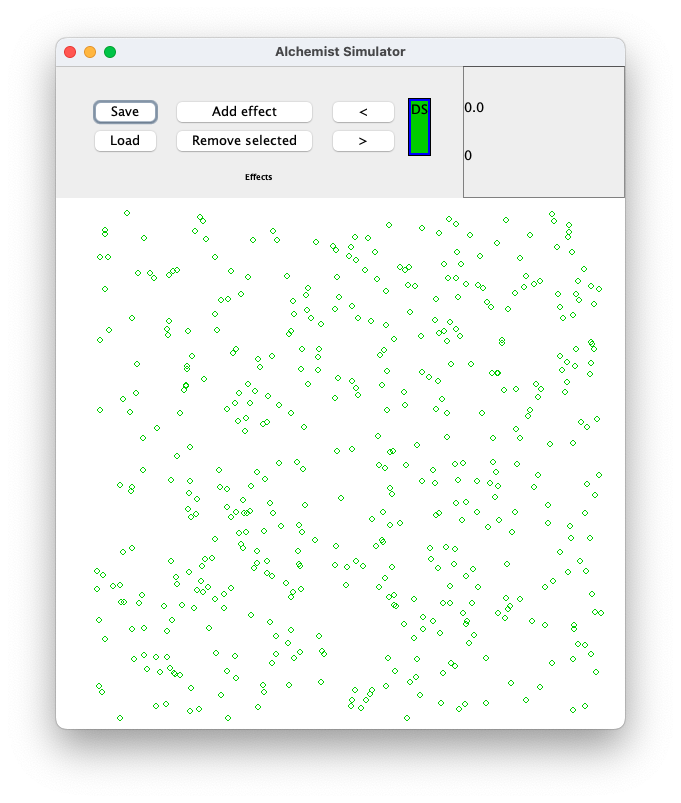
\includegraphics[width=0.32\textwidth]{figures/small0.png}} 
    \subfigure[]{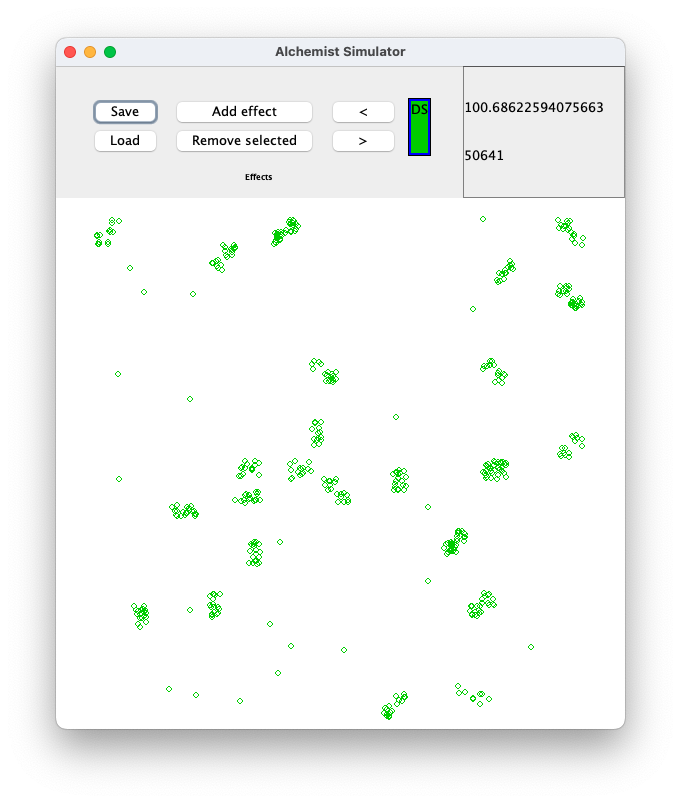
\includegraphics[width=0.32\textwidth]{figures/small100.png}} 
    \subfigure[]{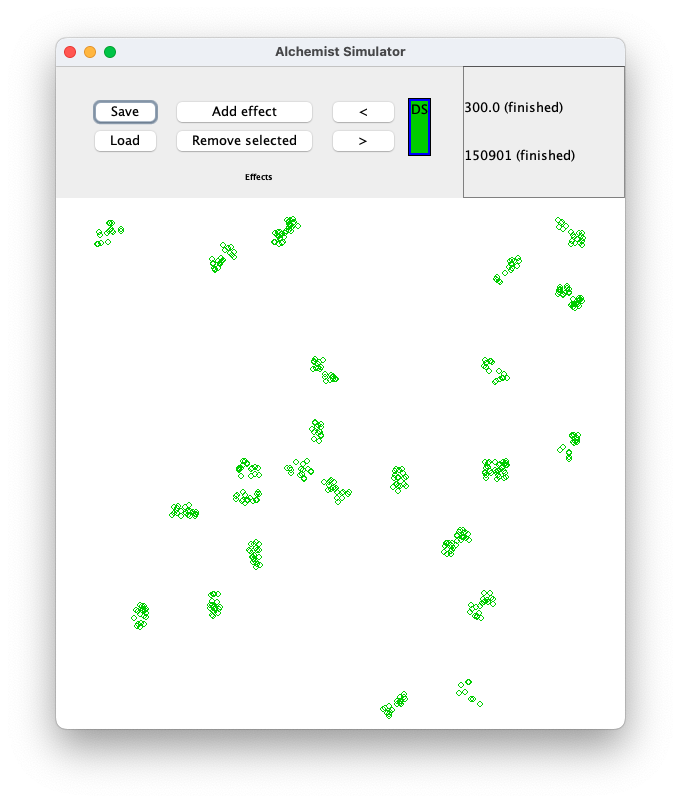
\includegraphics[width=0.32\textwidth]{figures/smallF.png}}
    \caption{(a) Inizio (b) Dopo 100 secondi (c) Dopo 300 secondi}\label{fig:sim5}
\end{figure}

\subsection{Risultati}
I risultati che si possono osservare dalle simulazioni eseguite sono i seguenti:
le simulazioni 1\space\ref{sim1} e 2\space\ref{sim2}, che presentano un numero di nodi pari a 500, mostrano un andamento simile.
La loro differenza principale risiede nel valore di \texttt{diffusion}. Possiamo notare come, dopo 100 secondi,
in entrambe le simulazioni si osserva l'aggregazione, in più punti, dei nodi. La prima simulazione 
mostra un'aggregazione più ``densa'' rispetto alla seconda, in quanto sono presenti meno nodi ``liberi'' nello spazio.
Dopo 300 secondi la prima simulazione mostra che ogni nodo si è aggregato, mentre la seconda presenta ancora nodi vaganti.

Se confrontiamo le simulazioni 3\space\ref{sim3} e 4\space\ref{sim4}, che presentano gli stessi valori delle precedenti, ma con un numero di nodi pari a 100, possiamo osservare come, dopo 100 secondi,
la terza simulazione inizia a sviluppare delle aggregazioni, che vengono confermate e rafforzate dopo 300 secondi.
La quarta simulazione, invece non presenta alcun fenomeno di questo tipo.

Infine, la simulazione 5\space\ref{sim5}, che presenta un ambiente di dimensioni inferiori rispetto alle altre e 
valori più alti, mostra che l'aggregazione dei nodi è più rapida.

\section{Lavori futuri}
Come lavoro futuro si potrebbe modificare il modello per permettere all'utente di definire l'angolo di 
scoperta del feromone. Attualmente ogni nodo ``sniffa'' il feromone a 360 gradi, ma sarebbe interessante
poter definire un angolo di visuale, in modo da poter simulare comportamenti più realistici.